% -*-latex-*-
%\documentclass[handout]{beamer} 
\documentclass{beamer} 
\usepackage{etex}

\let\latexput\put
\usepackage{pictex}
\let\pictexput\put
\let\put\latexput

\newcommand{\G}{\mathcal{G}}
\newcommand{\Het}{\mathcal{H}}
\newcommand{\mutation}{$\cdot$} 
\newcommand{\OR}{\;\hbox{or}\;}
\newcommand{\AND}{\;\&\;}
\newdimen\thusfar
\newdimen\plotht
\newdimen\plotwd
\newdimen\plotsp
\newdimen\xunit
\newdimen\yunit
\newdimen\offsety
\title{The History of Population Size from Whole Genomes}
\author{Alan R. Rogers}
\date{\today}
\begin{document}

\frame{\titlepage}

\begin{frame}
\frametitle{Simulated gene genealogy of a sample of size 50 from a
  population of constant size}
\centering% -*-latex-*-
\let\put\pictexput
\mbox{\beginpicture
\footnotesize
\setcoordinatesystem units <0.008\linewidth, 0.7mm>
%Sample size = 50
\setplotarea x from 0 to 100, y from 0.000000 to 49.000000
\putrule from 0.000000 0.000000 to 1.203719 0.000000
\putrule from 0.000000 1.000000 to 0.829032 1.000000
\putrule from 0.000000 2.000000 to 0.829032 2.000000
\putrule from 0.829032 2.000000 to 0.829032 1.000000
\putrule from 0.829032 1.500000 to 0.957672 1.500000
\putrule from 0.000000 3.000000 to 0.092058 3.000000
\putrule from 0.000000 4.000000 to 0.092058 4.000000
\putrule from 0.092058 4.000000 to 0.092058 3.000000
\putrule from 0.092058 3.500000 to 0.957672 3.500000
\putrule from 0.957672 3.500000 to 0.957672 1.500000
\putrule from 0.957672 2.500000 to 1.203719 2.500000
\putrule from 1.203719 2.500000 to 1.203719 0.000000
\putrule from 1.203719 1.250000 to 18.039782 1.250000
\putrule from 0.000000 5.000000 to 0.051697 5.000000
\putrule from 0.000000 6.000000 to 0.027617 6.000000
\putrule from 0.000000 7.000000 to 0.027617 7.000000
\putrule from 0.027617 7.000000 to 0.027617 6.000000
\putrule from 0.027617 6.500000 to 0.051697 6.500000
\putrule from 0.051697 6.500000 to 0.051697 5.000000
\putrule from 0.051697 5.750000 to 1.552095 5.750000
\putrule from 0.000000 8.000000 to 1.552094 8.000000
\putrule from 1.552094 8.000000 to 1.552094 5.750000
\putrule from 1.552094 6.875000 to 18.039780 6.875000
\putrule from 18.039780 6.875000 to 18.039780 1.250000
\putrule from 18.039780 4.062500 to 26.290684 4.062500
\putrule from 0.000000 9.000000 to 0.815369 9.000000
\putrule from 0.000000 10.000000 to 0.815369 10.000000
\putrule from 0.815369 10.000000 to 0.815369 9.000000
\putrule from 0.815369 9.500000 to 1.872993 9.500000
\putrule from 0.000000 11.000000 to 1.226610 11.000000
\putrule from 0.000000 12.000000 to 1.226610 12.000000
\putrule from 1.226610 12.000000 to 1.226610 11.000000
\putrule from 1.226610 11.500000 to 1.872992 11.500000
\putrule from 1.872992 11.500000 to 1.872992 9.500000
\putrule from 1.872992 10.500000 to 2.967822 10.500000
\putrule from 0.000000 13.000000 to 0.225777 13.000000
\putrule from 0.000000 14.000000 to 0.143829 14.000000
\putrule from 0.000000 15.000000 to 0.143829 15.000000
\putrule from 0.143829 15.000000 to 0.143829 14.000000
\putrule from 0.143829 14.500000 to 0.225777 14.500000
\putrule from 0.225777 14.500000 to 0.225777 13.000000
\putrule from 0.225777 13.750000 to 1.159578 13.750000
\putrule from 0.000000 16.000000 to 0.746065 16.000000
\putrule from 0.000000 17.000000 to 0.063148 17.000000
\putrule from 0.000000 18.000000 to 0.063148 18.000000
\putrule from 0.063148 18.000000 to 0.063148 17.000000
\putrule from 0.063148 17.500000 to 0.746065 17.500000
\putrule from 0.746065 17.500000 to 0.746065 16.000000
\putrule from 0.746065 16.750000 to 1.159578 16.750000
\putrule from 1.159578 16.750000 to 1.159578 13.750000
\putrule from 1.159578 15.250000 to 2.967822 15.250000
\putrule from 2.967822 15.250000 to 2.967822 10.500000
\putrule from 2.967822 12.875000 to 8.711625 12.875000
\putrule from 0.000000 19.000000 to 0.266543 19.000000
\putrule from 0.000000 20.000000 to 0.266543 20.000000
\putrule from 0.266543 20.000000 to 0.266543 19.000000
\putrule from 0.266543 19.500000 to 6.565042 19.500000
\putrule from 0.000000 21.000000 to 6.565042 21.000000
\putrule from 6.565042 21.000000 to 6.565042 19.500000
\putrule from 6.565042 20.250000 to 8.711626 20.250000
\putrule from 8.711626 20.250000 to 8.711626 12.875000
\putrule from 8.711626 16.562500 to 26.290686 16.562500
\putrule from 26.290686 16.562500 to 26.290686 4.062500
\putrule from 26.290686 10.312500 to 94.512634 10.312500
\putrule from 0.000000 22.000000 to 1.637721 22.000000
\putrule from 0.000000 23.000000 to 0.708858 23.000000
\putrule from 0.000000 24.000000 to 0.065136 24.000000
\putrule from 0.000000 25.000000 to 0.065136 25.000000
\putrule from 0.065136 25.000000 to 0.065136 24.000000
\putrule from 0.065136 24.500000 to 0.708858 24.500000
\putrule from 0.708858 24.500000 to 0.708858 23.000000
\putrule from 0.708858 23.750000 to 1.637721 23.750000
\putrule from 1.637721 23.750000 to 1.637721 22.000000
\putrule from 1.637721 22.875000 to 8.000084 22.875000
\putrule from 0.000000 26.000000 to 0.709645 26.000000
\putrule from 0.000000 27.000000 to 0.520728 27.000000
\putrule from 0.000000 28.000000 to 0.520728 28.000000
\putrule from 0.520728 28.000000 to 0.520728 27.000000
\putrule from 0.520728 27.500000 to 0.709645 27.500000
\putrule from 0.709645 27.500000 to 0.709645 26.000000
\putrule from 0.709645 26.750000 to 4.640732 26.750000
\putrule from 0.000000 29.000000 to 0.401201 29.000000
\putrule from 0.000000 30.000000 to 0.401201 30.000000
\putrule from 0.401201 30.000000 to 0.401201 29.000000
\putrule from 0.401201 29.500000 to 1.739993 29.500000
\putrule from 0.000000 31.000000 to 0.090187 31.000000
\putrule from 0.000000 32.000000 to 0.090187 32.000000
\putrule from 0.090187 32.000000 to 0.090187 31.000000
\putrule from 0.090187 31.500000 to 0.719749 31.500000
\putrule from 0.000000 33.000000 to 0.719749 33.000000
\putrule from 0.719749 33.000000 to 0.719749 31.500000
\putrule from 0.719749 32.250000 to 1.739993 32.250000
\putrule from 1.739993 32.250000 to 1.739993 29.500000
\putrule from 1.739993 30.875000 to 1.965272 30.875000
\putrule from 0.000000 34.000000 to 1.965272 34.000000
\putrule from 1.965272 34.000000 to 1.965272 30.875000
\putrule from 1.965272 32.437500 to 2.329356 32.437500
\putrule from 0.000000 35.000000 to 0.289964 35.000000
\putrule from 0.000000 36.000000 to 0.289964 36.000000
\putrule from 0.289964 36.000000 to 0.289964 35.000000
\putrule from 0.289964 35.500000 to 1.377131 35.500000
\putrule from 0.000000 37.000000 to 1.377131 37.000000
\putrule from 1.377131 37.000000 to 1.377131 35.500000
\putrule from 1.377131 36.250000 to 2.329356 36.250000
\putrule from 2.329356 36.250000 to 2.329356 32.437500
\putrule from 2.329356 34.343750 to 3.124661 34.343750
\putrule from 0.000000 38.000000 to 1.675222 38.000000
\putrule from 0.000000 39.000000 to 1.675222 39.000000
\putrule from 1.675222 39.000000 to 1.675222 38.000000
\putrule from 1.675222 38.500000 to 2.334833 38.500000
\putrule from 0.000000 40.000000 to 0.595711 40.000000
\putrule from 0.000000 41.000000 to 0.474361 41.000000
\putrule from 0.000000 42.000000 to 0.474361 42.000000
\putrule from 0.474361 42.000000 to 0.474361 41.000000
\putrule from 0.474361 41.500000 to 0.595711 41.500000
\putrule from 0.595711 41.500000 to 0.595711 40.000000
\putrule from 0.595711 40.750000 to 2.334833 40.750000
\putrule from 2.334833 40.750000 to 2.334833 38.500000
\putrule from 2.334833 39.625000 to 3.124661 39.625000
\putrule from 3.124661 39.625000 to 3.124661 34.343750
\putrule from 3.124661 36.984375 to 4.640732 36.984375
\putrule from 4.640732 36.984375 to 4.640732 26.750000
\putrule from 4.640732 31.867188 to 8.000085 31.867188
\putrule from 8.000085 31.867188 to 8.000085 22.875000
\putrule from 8.000085 27.371094 to 18.302837 27.371094
\putrule from 0.000000 43.000000 to 0.184519 43.000000
\putrule from 0.000000 44.000000 to 0.184519 44.000000
\putrule from 0.184519 44.000000 to 0.184519 43.000000
\putrule from 0.184519 43.500000 to 0.532117 43.500000
\putrule from 0.000000 45.000000 to 0.532117 45.000000
\putrule from 0.532117 45.000000 to 0.532117 43.500000
\putrule from 0.532117 44.250000 to 3.226239 44.250000
\putrule from 0.000000 46.000000 to 0.111898 46.000000
\putrule from 0.000000 47.000000 to 0.111898 47.000000
\putrule from 0.111898 47.000000 to 0.111898 46.000000
\putrule from 0.111898 46.500000 to 3.226239 46.500000
\putrule from 3.226239 46.500000 to 3.226239 44.250000
\putrule from 3.226239 45.375000 to 3.417443 45.375000
\putrule from 0.000000 48.000000 to 1.517669 48.000000
\putrule from 0.000000 49.000000 to 1.517669 49.000000
\putrule from 1.517669 49.000000 to 1.517669 48.000000
\putrule from 1.517669 48.500000 to 3.417442 48.500000
\putrule from 3.417442 48.500000 to 3.417442 45.375000
\putrule from 3.417442 46.937500 to 18.302837 46.937500
\putrule from 18.302837 46.937500 to 18.302837 27.371094
\putrule from 18.302837 37.154297 to 94.512634 37.154297
\putrule from 94.512634 37.154297 to 94.512634 10.312500
\putrule from 94.512634 23.733398 to 100 23.733398
\endpicture}
\let\put\latexput
\\

\bigskip

\begin{itemize}
\item Short terminal branches; long basal ones.
\item Large samples tell us about recent past.
\item Not necessary for ancient past.
\end{itemize}
\end{frame}

\begin{frame}
\begin{columns}
\column{0.5\textwidth}
% -*-latex-*-
%
%%%%%%%%%%%%%% Tree in PicTeX Format %%%%%%%%%%%%%%
%
%Sample size   = 50
%Mutation rate = 1
%     theta         mn        tau          K
%  100.0000     0.0000     8.0000          1
%    0.1000     0.0000        Inf          1
%maxmm=15.000000 maxtau=8.800000 maxtree=8.958047 maxx=15.000000
\newdimen\offsety
\newdimen\yunit
\newdimen\xunit
\newdimen\thusfar
\newdimen\plotht
\newdimen\plotwd
\newdimen\plotsp
\thusfar=0.000000in  % Keeps track of what's above
\plotht=1.400000in   % Height of each plot
\plotwd=4.000000in   % Width of each plot
\plotsp=0.500000in   % Spacing between plots
\begin{figure}
\begin{center}
\mbox{\beginpicture
\def\mutation{\tiny$\bullet$}
\small
\valuestolabelleading=.4\baselineskip
\headingtoplotskip=0.4\baselineskip
%
%%%%%%%%%%%%%% Population size %%%%%%%%%%%%%%
%
\yunit=\plotht
\xunit=\plotwd
\Divide <\xunit> by <15.000000pt> forming <\xunit>
\Divide <\yunit> by <120.000008pt> forming <\yunit>
\advance\thusfar by \plotht
\advance\thusfar by \plotsp
\Divide <\thusfar> by <\yunit> forming <\offsety>
\placevalueinpts of <\offsety> in {\mktree_tmp}
\setcoordinatesystem units <\xunit, \yunit> point at 0 {\mktree_tmp}
\setplotarea x from 0.000000 to 15.000000, y from 0.000000 to 120.000008
\advance\thusfar by 0.030000\plotht
\axis left label {\lines{Population\cr size}} /
\axis bottom shiftedto y=-3.600000
    label {Mutational time before present}
    ticks numbered from 0 to 15 by 5 /
\putrule from 0.000000 100.000000 to 8.000000 100.000000
\putrule from 8.000000 100.000000 to 8.000000 0.100000
\putrule from 8.000000 0.100000 to 15.000000 0.100000
%
%%%%%%%%%%%%%% Gene Genealogy %%%%%%%%%%%%%%
%
\yunit=\plotht
\xunit=\plotwd
\Divide <\xunit> by <15.000000pt> forming <\xunit>
\Divide <\yunit> by <49.000000pt> forming <\yunit>
\advance\thusfar by \plotht
\advance\thusfar by \plotsp
\Divide <\thusfar> by <\yunit> forming <\offsety>
\placevalueinpts of <\offsety> in {\mktree_tmp}
\setcoordinatesystem units <\xunit, \yunit> point at 0 {\mktree_tmp}
\setplotarea x from 0.000000 to 15.000000, y from 0.000000 to 49.000000
\axis left invisible label {\lines{Gene\cr genealogy}} /
\axis bottom invisible
     label {Mutational time before present} /
\putrule from 0.000000 0.000000 to 4.836251 0.000000
\put {\mutation} at 3.452781 0.000000
\put {\mutation} at 1.952839 0.000000
\put {\mutation} at 1.410723 0.000000
\putrule from 0.000000 1.000000 to 4.836251 1.000000
\put {\mutation} at 1.799608 1.000000
\putrule from 4.836251 1.000000 to 4.836251 0.000000
\putrule from 4.836251 0.500000 to 8.000854 0.500000
\put {\mutation} at 7.587026 0.500000
\put {\mutation} at 6.529379 0.500000
\put {\mutation} at 6.834705 0.500000
\putrule from 0.000000 2.000000 to 1.462832 2.000000
\put {\mutation} at 1.328440 2.000000
\put {\mutation} at 0.857991 2.000000
\putrule from 0.000000 3.000000 to 0.044562 3.000000
\putrule from 0.000000 4.000000 to 0.044562 4.000000
\putrule from 0.044562 4.000000 to 0.044562 3.000000
\putrule from 0.044562 3.500000 to 1.462832 3.500000
\put {\mutation} at 0.704485 3.500000
\putrule from 1.462832 3.500000 to 1.462832 2.000000
\putrule from 1.462832 2.750000 to 8.000854 2.750000
\put {\mutation} at 6.041394 2.750000
\put {\mutation} at 1.724101 2.750000
\put {\mutation} at 4.480876 2.750000
\put {\mutation} at 6.547650 2.750000
\put {\mutation} at 4.466406 2.750000
\putrule from 8.000854 2.750000 to 8.000854 0.500000
\putrule from 8.000854 1.625000 to 8.025000 1.625000
\putrule from 0.000000 5.000000 to 8.002358 5.000000
\put {\mutation} at 3.926434 5.000000
\put {\mutation} at 6.075176 5.000000
\put {\mutation} at 6.939764 5.000000
\put {\mutation} at 5.579136 5.000000
\putrule from 0.000000 6.000000 to 8.002358 6.000000
\put {\mutation} at 2.878085 6.000000
\put {\mutation} at 6.922358 6.000000
\put {\mutation} at 4.400364 6.000000
\putrule from 8.002358 6.000000 to 8.002358 5.000000
\putrule from 8.002358 5.500000 to 8.024999 5.500000
\putrule from 8.024999 5.500000 to 8.024999 1.625000
\putrule from 8.024999 3.562500 to 8.050393 3.562500
\putrule from 0.000000 7.000000 to 6.710411 7.000000
\putrule from 0.000000 8.000000 to 6.710411 8.000000
\put {\mutation} at 3.783755 8.000000
\putrule from 6.710411 8.000000 to 6.710411 7.000000
\putrule from 6.710411 7.500000 to 8.050393 7.500000
\put {\mutation} at 7.094459 7.500000
\putrule from 8.050393 7.500000 to 8.050393 3.562500
\putrule from 8.050393 5.531250 to 8.143679 5.531250
\putrule from 0.000000 9.000000 to 8.142600 9.000000
\put {\mutation} at 2.906895 9.000000
\putrule from 0.000000 10.000000 to 3.547134 10.000000
\put {\mutation} at 3.498341 10.000000
\putrule from 0.000000 11.000000 to 0.187752 11.000000
\putrule from 0.000000 12.000000 to 0.187752 12.000000
\putrule from 0.187752 12.000000 to 0.187752 11.000000
\putrule from 0.187752 11.500000 to 0.447217 11.500000
\putrule from 0.000000 13.000000 to 0.447217 13.000000
\putrule from 0.447217 13.000000 to 0.447217 11.500000
\putrule from 0.447217 12.250000 to 3.547134 12.250000
\put {\mutation} at 2.420029 12.250000
\putrule from 3.547134 12.250000 to 3.547134 10.000000
\putrule from 3.547134 11.125000 to 8.054446 11.125000
\put {\mutation} at 4.960887 11.125000
\put {\mutation} at 5.290615 11.125000
\put {\mutation} at 4.422930 11.125000
\put {\mutation} at 5.067940 11.125000
\putrule from 0.000000 14.000000 to 1.629022 14.000000
\putrule from 0.000000 15.000000 to 1.629022 15.000000
\put {\mutation} at 1.344186 15.000000
\putrule from 1.629022 15.000000 to 1.629022 14.000000
\putrule from 1.629022 14.500000 to 4.052386 14.500000
\put {\mutation} at 3.168806 14.500000
\put {\mutation} at 2.324489 14.500000
\put {\mutation} at 1.735080 14.500000
\putrule from 0.000000 16.000000 to 0.052486 16.000000
\putrule from 0.000000 17.000000 to 0.052486 17.000000
\putrule from 0.052486 17.000000 to 0.052486 16.000000
\putrule from 0.052486 16.500000 to 3.664456 16.500000
\put {\mutation} at 0.727443 16.500000
\putrule from 0.000000 18.000000 to 1.215439 18.000000
\putrule from 0.000000 19.000000 to 0.378657 19.000000
\put {\mutation} at 0.309676 19.000000
\putrule from 0.000000 20.000000 to 0.378657 20.000000
\putrule from 0.378657 20.000000 to 0.378657 19.000000
\putrule from 0.378657 19.500000 to 1.215439 19.500000
\putrule from 1.215439 19.500000 to 1.215439 18.000000
\putrule from 1.215439 18.750000 to 3.626270 18.750000
\put {\mutation} at 3.552026 18.750000
\putrule from 0.000000 21.000000 to 0.102288 21.000000
\putrule from 0.000000 22.000000 to 0.102288 22.000000
\putrule from 0.102288 22.000000 to 0.102288 21.000000
\putrule from 0.102288 21.500000 to 1.725883 21.500000
\put {\mutation} at 0.847011 21.500000
\putrule from 0.000000 23.000000 to 1.725883 23.000000
\putrule from 1.725883 23.000000 to 1.725883 21.500000
\putrule from 1.725883 22.250000 to 2.602657 22.250000
\putrule from 0.000000 24.000000 to 2.602657 24.000000
\put {\mutation} at 0.447969 24.000000
\putrule from 2.602657 24.000000 to 2.602657 22.250000
\putrule from 2.602657 23.125000 to 3.626270 23.125000
\put {\mutation} at 2.815562 23.125000
\putrule from 3.626270 23.125000 to 3.626270 18.750000
\putrule from 3.626270 20.937500 to 3.664456 20.937500
\putrule from 3.664456 20.937500 to 3.664456 16.500000
\putrule from 3.664456 18.718750 to 4.052386 18.718750
\putrule from 4.052386 18.718750 to 4.052386 14.500000
\putrule from 4.052386 16.609375 to 8.028200 16.609375
\put {\mutation} at 4.464513 16.609375
\put {\mutation} at 4.202519 16.609375
\putrule from 0.000000 25.000000 to 8.001245 25.000000
\put {\mutation} at 5.238211 25.000000
\put {\mutation} at 0.597891 25.000000
\put {\mutation} at 4.546607 25.000000
\put {\mutation} at 7.491570 25.000000
\putrule from 0.000000 26.000000 to 6.076888 26.000000
\put {\mutation} at 3.655453 26.000000
\put {\mutation} at 5.642963 26.000000
\put {\mutation} at 4.709704 26.000000
\put {\mutation} at 2.365931 26.000000
\put {\mutation} at 1.423714 26.000000
\putrule from 0.000000 27.000000 to 6.076888 27.000000
\put {\mutation} at 1.023258 27.000000
\put {\mutation} at 5.642505 27.000000
\put {\mutation} at 4.191251 27.000000
\putrule from 6.076888 27.000000 to 6.076888 26.000000
\putrule from 6.076888 26.500000 to 8.001245 26.500000
\put {\mutation} at 6.117506 26.500000
\put {\mutation} at 6.742373 26.500000
\putrule from 8.001245 26.500000 to 8.001245 25.000000
\putrule from 8.001245 25.750000 to 8.028199 25.750000
\putrule from 8.028199 25.750000 to 8.028199 16.609375
\putrule from 8.028199 21.179688 to 8.039419 21.179688
\putrule from 0.000000 28.000000 to 3.924574 28.000000
\put {\mutation} at 3.547138 28.000000
\put {\mutation} at 1.944984 28.000000
\put {\mutation} at 0.489562 28.000000
\put {\mutation} at 3.400585 28.000000
\put {\mutation} at 1.640684 28.000000
\putrule from 0.000000 29.000000 to 3.924574 29.000000
\put {\mutation} at 3.178097 29.000000
\put {\mutation} at 0.166115 29.000000
\put {\mutation} at 2.098241 29.000000
\put {\mutation} at 2.261311 29.000000
\putrule from 3.924574 29.000000 to 3.924574 28.000000
\putrule from 3.924574 28.500000 to 8.027688 28.500000
\put {\mutation} at 5.267450 28.500000
\put {\mutation} at 3.949556 28.500000
\put {\mutation} at 4.231240 28.500000
\putrule from 0.000000 30.000000 to 5.551525 30.000000
\put {\mutation} at 5.400300 30.000000
\put {\mutation} at 0.819270 30.000000
\putrule from 0.000000 31.000000 to 0.158670 31.000000
\putrule from 0.000000 32.000000 to 0.158670 32.000000
\putrule from 0.158670 32.000000 to 0.158670 31.000000
\putrule from 0.158670 31.500000 to 2.987517 31.500000
\put {\mutation} at 1.895310 31.500000
\putrule from 0.000000 33.000000 to 2.987517 33.000000
\put {\mutation} at 2.159181 33.000000
\putrule from 2.987517 33.000000 to 2.987517 31.500000
\putrule from 2.987517 32.250000 to 5.551525 32.250000
\put {\mutation} at 4.102941 32.250000
\putrule from 5.551525 32.250000 to 5.551525 30.000000
\putrule from 5.551525 31.125000 to 8.000154 31.125000
\putrule from 0.000000 34.000000 to 1.032043 34.000000
\put {\mutation} at 0.568913 34.000000
\putrule from 0.000000 35.000000 to 1.032043 35.000000
\putrule from 1.032043 35.000000 to 1.032043 34.000000
\putrule from 1.032043 34.500000 to 3.099934 34.500000
\putrule from 0.000000 36.000000 to 0.538050 36.000000
\put {\mutation} at 0.228365 36.000000
\putrule from 0.000000 37.000000 to 0.538050 37.000000
\putrule from 0.538050 37.000000 to 0.538050 36.000000
\putrule from 0.538050 36.500000 to 3.099934 36.500000
\put {\mutation} at 0.649459 36.500000
\put {\mutation} at 0.877839 36.500000
\putrule from 3.099934 36.500000 to 3.099934 34.500000
\putrule from 3.099934 35.500000 to 8.000154 35.500000
\put {\mutation} at 5.197902 35.500000
\put {\mutation} at 3.883441 35.500000
\put {\mutation} at 7.879986 35.500000
\putrule from 8.000154 35.500000 to 8.000154 31.125000
\putrule from 8.000154 33.312500 to 8.009798 33.312500
\putrule from 0.000000 38.000000 to 8.004445 38.000000
\put {\mutation} at 2.441105 38.000000
\put {\mutation} at 5.712032 38.000000
\put {\mutation} at 5.006180 38.000000
\put {\mutation} at 0.229807 38.000000
\putrule from 0.000000 39.000000 to 1.899162 39.000000
\put {\mutation} at 1.401599 39.000000
\putrule from 0.000000 40.000000 to 1.899162 40.000000
\put {\mutation} at 1.448626 40.000000
\putrule from 1.899162 40.000000 to 1.899162 39.000000
\putrule from 1.899162 39.500000 to 4.666477 39.500000
\put {\mutation} at 4.625469 39.500000
\putrule from 0.000000 41.000000 to 4.666476 41.000000
\putrule from 4.666476 41.000000 to 4.666476 39.500000
\putrule from 4.666476 40.250000 to 8.004445 40.250000
\put {\mutation} at 7.990844 40.250000
\putrule from 8.004445 40.250000 to 8.004445 38.000000
\putrule from 8.004445 39.125000 to 8.005302 39.125000
\putrule from 0.000000 42.000000 to 8.003333 42.000000
\put {\mutation} at 1.262157 42.000000
\put {\mutation} at 4.937531 42.000000
\put {\mutation} at 1.317544 42.000000
\put {\mutation} at 2.173934 42.000000
\putrule from 0.000000 43.000000 to 5.748858 43.000000
\put {\mutation} at 1.932616 43.000000
\put {\mutation} at 4.137879 43.000000
\put {\mutation} at 0.070606 43.000000
\putrule from 0.000000 44.000000 to 1.387771 44.000000
\put {\mutation} at 0.905631 44.000000
\put {\mutation} at 1.134355 44.000000
\putrule from 0.000000 45.000000 to 1.387771 45.000000
\put {\mutation} at 0.747416 45.000000
\put {\mutation} at 0.027540 45.000000
\putrule from 1.387771 45.000000 to 1.387771 44.000000
\putrule from 1.387771 44.500000 to 5.324390 44.500000
\putrule from 0.000000 46.000000 to 3.905474 46.000000
\put {\mutation} at 0.372534 46.000000
\putrule from 0.000000 47.000000 to 0.086328 47.000000
\putrule from 0.000000 48.000000 to 0.086328 48.000000
\putrule from 0.086328 48.000000 to 0.086328 47.000000
\putrule from 0.086328 47.500000 to 0.503535 47.500000
\putrule from 0.000000 49.000000 to 0.503535 49.000000
\putrule from 0.503535 49.000000 to 0.503535 47.500000
\putrule from 0.503535 48.250000 to 3.905474 48.250000
\put {\mutation} at 1.573812 48.250000
\put {\mutation} at 1.576257 48.250000
\put {\mutation} at 0.759165 48.250000
\putrule from 3.905474 48.250000 to 3.905474 46.000000
\putrule from 3.905474 47.125000 to 5.324390 47.125000
\putrule from 5.324390 47.125000 to 5.324390 44.500000
\putrule from 5.324390 45.812500 to 5.748859 45.812500
\putrule from 5.748859 45.812500 to 5.748859 43.000000
\putrule from 5.748859 44.406250 to 8.003334 44.406250
\put {\mutation} at 6.363234 44.406250
\put {\mutation} at 7.245713 44.406250
\putrule from 8.003334 44.406250 to 8.003334 42.000000
\putrule from 8.003334 43.203125 to 8.005303 43.203125
\putrule from 8.005303 43.203125 to 8.005303 39.125000
\putrule from 8.005303 41.164062 to 8.009798 41.164062
\putrule from 8.009798 41.164062 to 8.009798 33.312500
\putrule from 8.009798 37.238281 to 8.027688 37.238281
\putrule from 8.027688 37.238281 to 8.027688 28.500000
\putrule from 8.027688 32.869141 to 8.039419 32.869141
\putrule from 8.039419 32.869141 to 8.039419 21.179688
\putrule from 8.039419 27.024414 to 8.054446 27.024414
\putrule from 8.054446 27.024414 to 8.054446 11.125000
\putrule from 8.054446 19.074707 to 8.142601 19.074707
\putrule from 8.142601 19.074707 to 8.142601 9.000000
\putrule from 8.142601 14.037354 to 8.143680 14.037354
\putrule from 8.143680 14.037354 to 8.143680 5.531250
\putrule from 8.143680 9.784302 to 15.000000 9.784302
%
%%%%%%%%%%%%%% Mismatch Distribution %%%%%%%%%%%%%%
%
\yunit=\plotht
\xunit=\plotwd
\Divide <\xunit> by <15.000000pt> forming <\xunit>
\Divide <\yunit> by <0.158367pt> forming <\yunit>
\advance\thusfar by \plotht
\advance\thusfar by \plotsp
\Divide <\thusfar> by <\yunit> forming <\offsety>
\placevalueinpts of <\offsety> in {\mktree_tmp}
\setcoordinatesystem units <\xunit, \yunit> point at 0 {\mktree_tmp}
\setplotarea x from 0.000000 to 15.000000, y from 0.000000 to 0.158367
\axis left label {\lines{Mismatch\cr distribution}} /
\axis bottom
   label {Pairwise differences}
   ticks numbered from 0 to 15 by 5 /
\multiput {$\circ$} at
 0 0.008980 1 0.007347 2 0.017959 3 0.028571 4 0.040816
 5 0.084082 6 0.109388 7 0.136327 8 0.158367 9 0.148571
 10 0.107755 11 0.080816 12 0.043265 13 0.019592 14 0.006531
 15 0.001633
/
\plot
 0 0.008980 1 0.007347 2 0.017959 3 0.028571 4 0.040816
 5 0.084082 6 0.109388 7 0.136327 8 0.158367 9 0.148571
 10 0.107755 11 0.080816 12 0.043265 13 0.019592 14 0.006531
 15 0.001633
/
\plotht=1.100000\plotht
%
%%%%%%%%%%%%%% Simulated site frequency spectrum %%%%%%%%%%%%%%
%
\yunit=\plotht
\xunit=\plotwd
\Divide <\xunit> by <49.000000pt> forming <\xunit>
\Divide <\yunit> by <0.653774pt> forming <\yunit>
\advance\thusfar by \plotht
\advance\thusfar by \plotsp
\Divide <\thusfar> by <\yunit> forming <\offsety>
\placevalueinpts of <\offsety> in {\mktree_tmp}
\setcoordinatesystem units <\xunit, \yunit> point at 0 {\mktree_tmp}
\setplotarea x from 0.000000 to 49.000000, y from 0.000000 to 0.653774
\axis left invisible label {\lines{Site\cr frequency\cr spectrum}} /
\axis bottom
   label {Frequency of mutant allele}
   ticks withvalues 0 1 / at 0 49 / /
\linethickness 1.2pt
\axis top /
\linethickness 0.4pt
\sethistograms
\plot 0 0 1 0.594340 2 0.179245 3 0.113208 4 0.075472
 5 0.000000 6 0.000000 7 0.018868 8 0.000000 9 0.000000
 10 0.000000 11 0.018868 12 0.000000 13 0.000000 14 0.000000
 15 0.000000 16 0.000000 17 0.000000 18 0.000000 19 0.000000
 20 0.000000 21 0.000000 22 0.000000 23 0.000000 24 0.000000
 25 0.000000 26 0.000000 27 0.000000 28 0.000000 29 0.000000
 30 0.000000 31 0.000000 32 0.000000 33 0.000000 34 0.000000
 35 0.000000 36 0.000000 37 0.000000 38 0.000000 39 0.000000
 40 0.000000 41 0.000000 42 0.000000 43 0.000000 44 0.000000
 45 0.000000 46 0.000000 47 0.000000 48 0.000000 49 0.000000
/
\setlinear
%
%%%%%%%%%%%%%% Neutral expectation of site freq spectrum %%%%%%%%%%%%%%
%
\multiput {$\bullet$} at 
     0.500000 0.223254  1.500000 0.111627  2.500000 0.074418  3.500000 0.0558135  4.500000 0.0446508
     5.500000 0.037209  6.500000 0.0318934  7.500000 0.0279067  8.500000 0.024806  9.500000 0.0223254
     10.500000 0.0202958  11.500000 0.0186045  12.500000 0.0171734  13.500000 0.0159467  14.500000 0.0148836
     15.500000 0.0139534  16.500000 0.0131326  17.500000 0.012403  18.500000 0.0117502  19.500000 0.0111627
     20.500000 0.0106311  21.500000 0.0101479  22.500000 0.00970669  23.500000 0.00930224  24.500000 0.00893015
     25.500000 0.00858669  26.500000 0.00826866  27.500000 0.00797335  28.500000 0.00769841  29.500000 0.0074418
     30.500000 0.00720174  31.500000 0.00697668  32.500000 0.00676527  33.500000 0.00656629  34.500000 0.00637868
     35.500000 0.0062015  36.500000 0.00603389  37.500000 0.0058751  38.500000 0.00572446  39.500000 0.00558135
     40.500000 0.00544522  41.500000 0.00531557  42.500000 0.00519195  43.500000 0.00507395  44.500000 0.0049612
     45.500000 0.00485335  46.500000 0.00475008  47.500000 0.00465112  48.500000 0.0045562
/
\endpicture}
\end{center}
mean pairwise difference: 7.783673
\end{figure}

\column{0.5\textwidth}
{\color{blue}Effect of a population explosion}\\

\bigskip

Middle: genealogy of 50 individuals; dots are mutations.\\

\bigskip

1 mutational diff per time unit

\bigskip

Bottom: $\circ$ = simulated data, line = theory.\\

\bigskip

Wave peaks at population expansion.\\
\end{columns}
\end{frame}

\begin{frame}
\frametitle{Skyline Plot}
\begin{columns}
\column{0.5\textwidth}
\includegraphics[width=\linewidth]{skyline.png}\\
\mbox{}\hfill\footnotesize (Drummond et al 2005)\\
\column{0.5\textwidth}
\begin{itemize}
\item Use mutations to estimate length of each interval.
\item Long intervals imply large population size.
\item Won't work with nuclear DNA: too few mutations per tree
\end{itemize}
\end{columns}
\end{frame}

\begin{frame}
\frametitle{Nuclear genome}

\begin{itemize}
\item Huge amounts of data.
\item Recombination makes previous methods unusable.
\end{itemize}
\end{frame}

\begin{frame}
\begin{columns}
\column{0.6\linewidth}
{\centering% -*-latex-*-
%
%%%%%%%%%%%%%% Tree in PicTeX Format %%%%%%%%%%%%%%
%
%Sample size   = 50
%Mutation rate = 1
%     theta         mn        tau          K
%  100.0000     0.0000     7.0000          1
%    1.0000     0.0000        Inf          1
%maxmm=20.000000 maxtau=7.700000 maxtree=8.748507 maxx=20.000000
%\newdimen\offsety
%\newdimen\yunit
%\newdimen\xunit
%\newdimen\thusfar
%\newdimen\plotht
%\newdimen\plotwd
%\newdimen\plotsp
\thusfar=0.000000in  % Keeps track of what's above
\plotht=0.8in   % Height of each plot
\plotwd=0.7\textwidth   % Width of each plot
\plotsp=0.500000in   % Spacing between plots
\let\put\pictexput
\mbox{\beginpicture
\def\mutation{\tiny$\bullet$}
\small
\valuestolabelleading=.2\baselineskip
\headingtoplotskip=0.4\baselineskip
%
%%%%%%%%%%%%%% Population size %%%%%%%%%%%%%%
%
\yunit=\plotht
\xunit=\plotwd
\Divide <\xunit> by <20.000000pt> forming <\xunit>
\Divide <\yunit> by <120.000008pt> forming <\yunit>
\advance\thusfar by \plotht
\advance\thusfar by \plotsp
\Divide <\thusfar> by <\yunit> forming <\offsety>
\placevalueinpts of <\offsety> in {\mktree_tmp}
\setcoordinatesystem units <\xunit, \yunit> point at 0 {\mktree_tmp}
\setplotarea x from 0.000000 to 20.000000, y from 0.000000 to 120.000008
\advance\thusfar by 0.030000\plotht
\axis left label {\lines{Population\cr size}} /
\axis bottom shiftedto y=-3.600000
    label {Mutational time before present}
    ticks numbered from 0 to 20 by 10 /
\putrule from 0.000000 100.000000 to 7.000000 100.000000
\putrule from 7.000000 100.000000 to 7.000000 1.000000
\putrule from 7.000000 1.000000 to 20.000000 1.000000
%
\plotht=1.300000\plotht
%
%%%%%%%%%%%%%% Simulated site frequency spectrum %%%%%%%%%%%%%%
%
\yunit=\plotht
\xunit=\plotwd
\Divide <\xunit> by <25.000000pt> forming <\xunit>
\Divide <\yunit> by <0.615596pt> forming <\yunit>
\advance\thusfar by \plotht
\advance\thusfar by \plotsp
\Divide <\thusfar> by <\yunit> forming <\offsety>
\placevalueinpts of <\offsety> in {\mktree_tmp}
\setcoordinatesystem units <\xunit, \yunit> point at 0 {\mktree_tmp}
\setplotarea x from 0.000000 to 25.000000, y from 0.000000 to 0.615596
\axis left invisible label {\lines{Site\cr frequency\cr spectrum}} /
\axis bottom
   label {Frequency of minor allele}
   ticks withvalues 0 {1/2} / at 0 25 / /
\linethickness 1.2pt
\axis top /
\linethickness 0.4pt
\sethistograms
\plot 0 0 1 0.559633 2 0.302752 3 0.018349 4 0.018349
 5 0.036697 6 0.018349 7 0.009174 8 0.009174 9 0.000000
 10 0.018349 11 0.000000 12 0.000000 13 0.000000 14 0.000000
 15 0.000000 16 0.000000 17 0.000000 18 0.000000 19 0.000000
 20 0.000000 21 0.000000 22 0.009174 23 0.000000 24 0.000000
 25 0.000000
/
\setlinear
%
%%%%%%%%%%%%%% Neutral expectation of site freq spectrum %%%%%%%%%%%%%%
%
\multiput {$\bullet$} at 
     0.500000 0.22781  1.500000 0.116278  2.500000 0.079168  3.500000 0.0606668  4.500000 0.049612
     5.500000 0.0422829  6.500000 0.0370854  7.500000 0.0332223  8.500000 0.0302512  9.500000 0.0279067
     10.500000 0.0260203  11.500000 0.0244796  12.500000 0.0232073  13.500000 0.0221482  14.500000 0.0212623
     15.500000 0.0205197  16.500000 0.0198978  17.500000 0.0193797  18.500000 0.0189519  19.500000 0.0186045
     20.500000 0.0183295  21.500000 0.0181213  22.500000 0.0179754  23.500000 0.0178889  24.500000 0.0178603
/
\endpicture}
\let\put\latexput
\\}
\column{0.4\linewidth}
\textcolor{blue}{\Large Site frequency spectrum}

\bigskip

The spectrum is useful with nuclear as well as mitochondrial DNA.

\bigskip

Population growth inflates the number of singletons. Bars show
simulated spectrum; filled circles show expectation under constant
population size.

\bigskip

To estimate history, we need a theory that works under complex
population histories.

\end{columns}
\end{frame}

\begin{frame}
  \frametitle{We do have such a theory}
  \begin{columns}
    \column{0.6\textwidth}
    \includegraphics[width=\linewidth]{Wooding-fig1.pdf}
    \column{0.4\textwidth}
    \raggedleft
    Row~1: 3 histories of population size

    \bigskip

    Row~2: Prob that there are $k$ lineages at time $t$ in a sample of
    size 5.

    \bigskip

    Row~3: Expected lengths each coalescent intervals.

    \bigskip

    Row~4: Expected spectrum

    \bigskip

    {\footnotesize Griffiths \& Tavar{\'e} (1998); Wooding \& Rogers (2002)\\}
  \end{columns}
\end{frame}  

\begin{frame}
\frametitle{$\partial$a$\partial$i: inferences from the site frequency spectrum}
\includegraphics[width=\linewidth]{gutenkunst.png}\\
\mbox{}\hfill\footnotesize(Gutenkunst et al 2009)\\
\end{frame}

\begin{frame}
\frametitle{Stairway plot (Liu \& Fu 2015)}

\begin{itemize}
\item uses site frequency spectrum
\item no need for phased data
\item can deal with samples of hundreds of individuals
\end{itemize}
\end{frame}

\begin{frame}
\frametitle{Stairway Plot results}
{\centering\includegraphics[height=0.8\textheight]{stairway.png}\\
\footnotesize 1000-Genomes data; (Liu \& Fu 2015)\\}
\end{frame}

\begin{frame}
\frametitle{Also: recombination is our friend}
\begin{columns}
\column{0.5\linewidth}
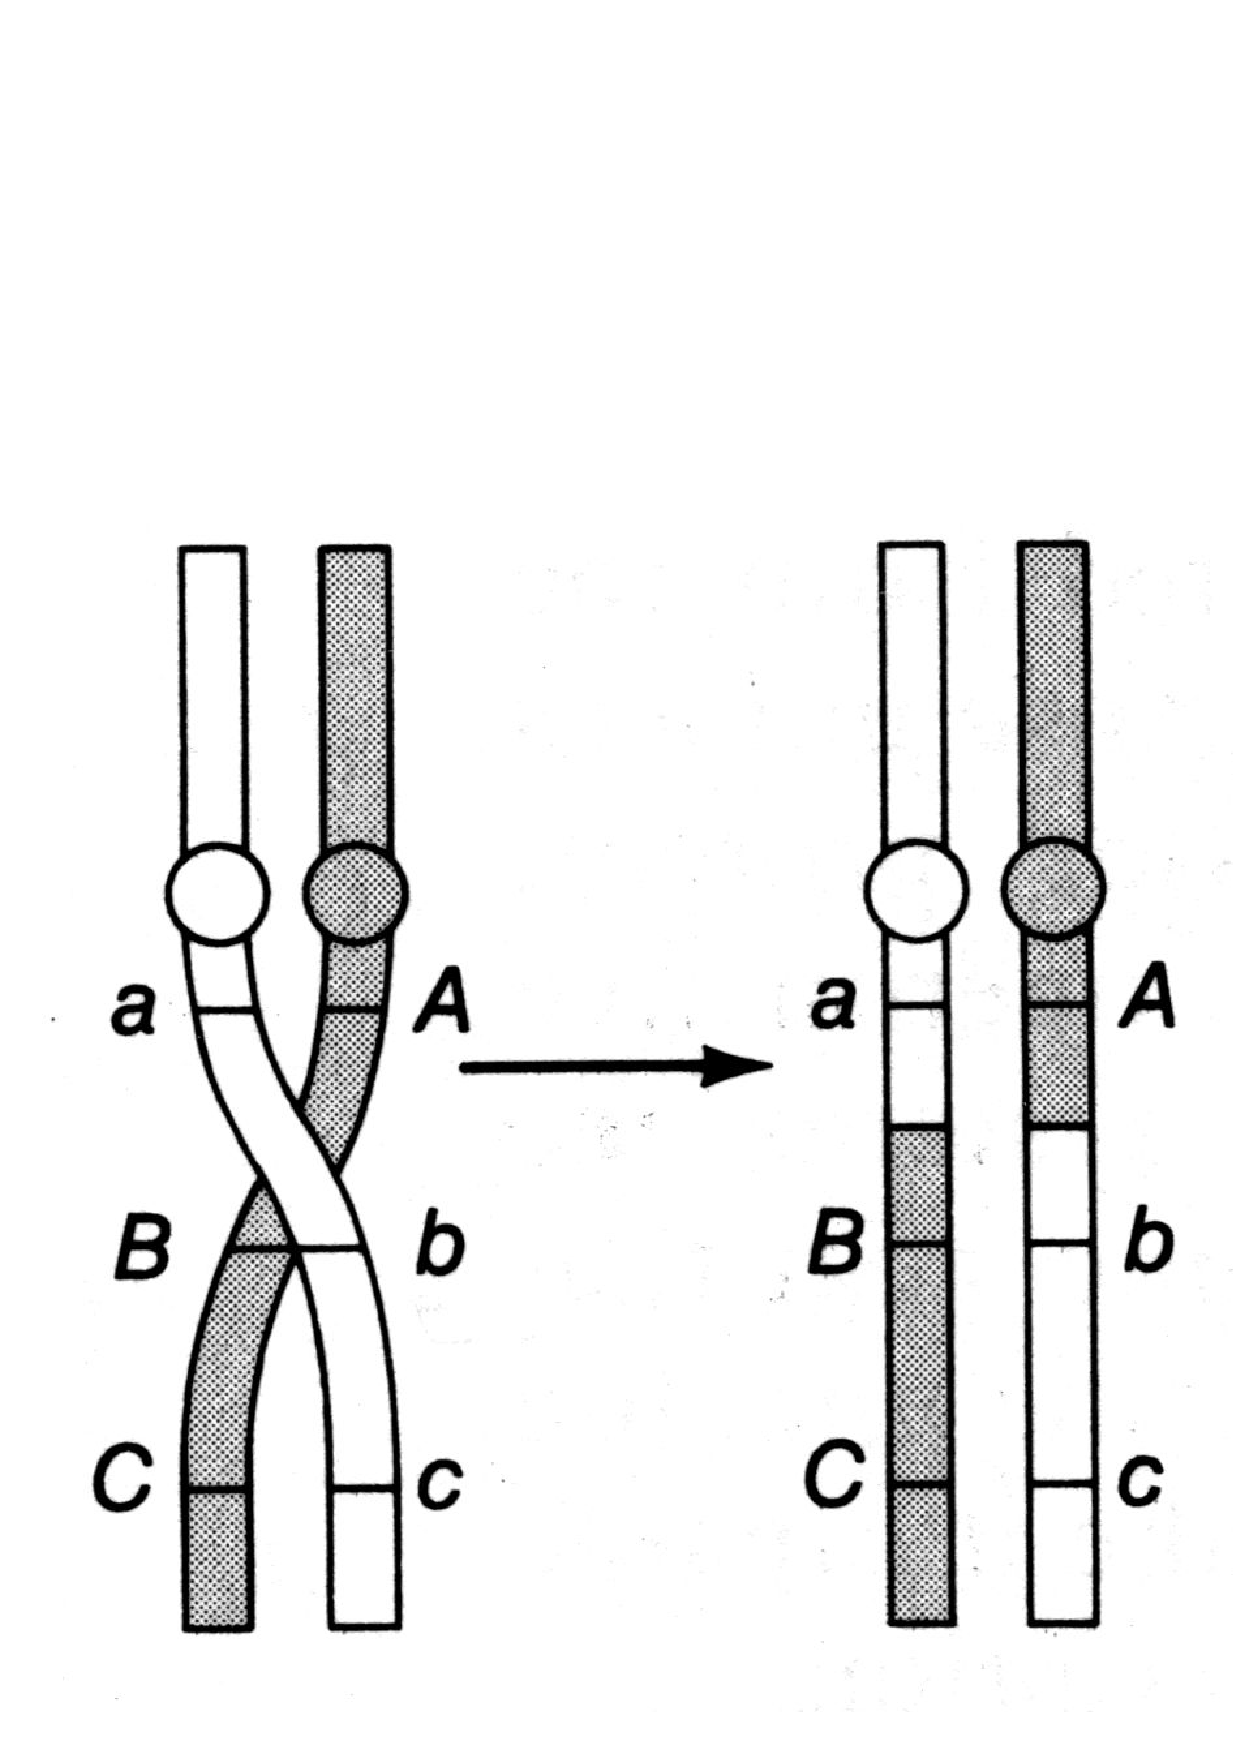
\includegraphics[width=\linewidth]{crossover.pdf}
\column{0.5\linewidth}
Useful data began to appear in about 2000.

\bigskip

Crossovers shuffle DNA

\bigskip

Each chromosome has many gene genealogies, which vary in length.
\end{columns}
\end{frame}

\begin{frame}
\frametitle{Two (hypothetical) loci in a single diploid genome}
{\centering% -*-latex-*-
%
%%%%%%%%%%%%%% Tree in PicTeX Format %%%%%%%%%%%%%%
%
%Sample size   = 2
%Do mutation = 1
%     theta         mn        tau          K
%   10.0000     0.0000        Inf          1
%maxmm=13.000000 maxtau=0.000000 maxtree=20.077202 maxx=20.077202
\let\put\pictexput
\mbox{\beginpicture
\def\mutation{\tiny$\bullet$}
\small
\valuestolabelleading=.4\baselineskip
\headingtoplotskip=0.4\baselineskip
%
%%%%%%%%%%%%%% Gene Genealogy %%%%%%%%%%%%%%
%
\setcoordinatesystem units <0.04\linewidth, 5ex> point at 0 0
\setplotarea x from 0 to 21, y from 0 to 3
\putrule from 0.000000 0.000000 to 18.252001 0.000000
\put {\mutation} at 12.763110 0.000000
\putrule from 0.000000 1.000000 to 18.252001 1.000000
\putrule from 18.252001 1.000000 to 18.252001 0.000000
\putrule from 18.252001 0.500000 to 21.000000 0.500000
\setbox0=\hbox{$\swarrow$}%
\put {$\swarrow$ \raise \ht0 \hbox{MRCA}}
   <0.3ex,0.3ex> [bl] at 18.252001 0.500000
%%%%%%%%%%%%%% Gene Genealogy %%%%%%%%%%%%%%
\putrule from 0.000000 2 to 5.022242 2
\putrule from 0.000000 3 to 5.022242 3
\putrule from 5.022242 3 to 5.022242 2
\putrule from 5.022242 2.500000 to 21 2.500000
\put {$\swarrow$ \raise \ht0 \hbox{MRCA}}
   <0.3ex,0.3ex> [bl] at 5.022242 2.500000
\endpicture}
\let\put\latexput
\\}

\bigskip

\begin{itemize}
\item MRCA: most recent common ancestor
\item Gene trees vary in length across the genome.
\item Mutation ({\tiny$\bullet$}) is more likely on a deep gene tree.
\end{itemize}
\end{frame}

\begin{frame}
\frametitle{MRCA varies along the chromosome}
{\centering\let\put\pictexput
\mbox{\beginpicture
\valuestolabelleading=\baselineskip
\tickstovaluesleading=0.5\baselineskip
\setcoordinatesystem units <0.08\linewidth, 4ex>
\setplotarea x from 0 to 10, y from 0 to 5
\axis left label {\lines{MRCA\cr (depth\cr of\cr gene\cr tree)\cr}} shiftedto x=-0.2 /
\axis bottom label {Chromosome} /
\plot 0 1 3 1 /
\plot 3 1 3 5 /
\plot 3 5 8 5 /
\plot 8 5 8 2 /
\plot 8 2 10 2 /
\multiput {$\circ$} at
0.6799798396333573 0
2.890620777308363 0
/
\multiput {$\circ$} at
7.505457071714459 0
7.528713066720229 0
7.897267201963705 0
6.742911647476683 0
3.3275297791190868 0
7.364327092162486 0
3.9876397186850117 0
3.2215719274426693 0
4.408645335396897 0
3.442186560410682 0
6.252505835935007 0
7.75256783425724 0
3.4390283173516893 0
7.06953802763253 0
6.3171251897670455 0
6.326735322130281 0
6.268346195910773 0
4.849079577128146 0
5.750625064351603 0
5.562974233930628 0
5.028000563562759 0
5.308758316103449 0
6.168788999194518 0
5.9297147962946 0
4.924798505853198 0
4.7522259027387275 0
4.107208387016464 0
3.0925392557402116 0
6.1218791634841745 0
6.829508710556947 0
5.01422434571627 0
3.8459313697644877 0
/
\multiput {$\circ$} at
9.863077990195158 0
8.71251946992873 0
8.55194529065689 0
8.683376626408 0
/
\endpicture}
\let\put\latexput
\\}
\begin{itemize}
%\item MRCA is depth of gene tree.
\item Circles: nucleotide sites that differ (are \emph{heterozygous})
  in a single diploid sample.
\item Heterozygous sites are denser where gene tree is deep.
\item Population size $\rightarrow$ length of
  MRCA segments and genetic variation within segments.
\item PSMC uses this pattern to estimate population history
\end{itemize}
\end{frame}

\begin{frame}
\frametitle{PSMC is accurate from 20~ky to 3~my ago.}
\centering
\includegraphics[width=\linewidth]{LiDurbin-sim.png}\\

\mbox{}\hfill{\small(Li and Durbin 2011)\\}
\end{frame}

\begin{frame}
\frametitle{PSMC estimates from autosomes}
\begin{columns}
\column{0.65\linewidth}
\includegraphics[width=\linewidth]{LiDurbin-esta.png}
\column{0.4\linewidth} $\uparrow$ 2~mya (origin of \emph{Homo});
$\uparrow$ 200~kya (origin of modern humans); $\uparrow$ 20~kya
(beginning of Holocene).
\end{columns}

\bigskip

Eurasian/African split 150~kya. 

\bigskip

African bottleneck short and shallow.
\end{frame}

\begin{frame}
\frametitle{PSMC estimates from X chromosomes}
\includegraphics[width=\linewidth]{LiDurbin-estb.png}
\end{frame}

\begin{frame}
\frametitle{PSMC with Neanderthal as well as Denisova}
\includegraphics[width=\linewidth]{Prufer-pophist.jpg}\\
\mbox{}\hfill\footnotesize(Pr{\"u}fer et al 2014)\\
\end{frame}

\begin{frame}
  \frametitle{All 3 high-coverage archaic genomes}
{\centering\includegraphics[width=0.9\linewidth]{Chagyrskaya-psmc.png}\\}

\bigskip

Horizontal axis shows time backwards from time of fossil's
death. Curves of younger fossil (Vindija) is shifted to right.\\
\mbox{}\hfill\footnotesize(Mafessoni et al 2022)\\
\end{frame}

\begin{frame}
  \frametitle{What if the population is subdivided? (part 1)}
  Suppose there are $K$ local groups, each of size $N$, which exchange
  migrants. We sample a single genome from some group. In the recent
  past, the hazard of a coalescent event is $h(t) = 1/2N$, and effective
  population size ($1/h(t)$) is $2N$.

  \bigskip

  Farther back in time, the ancestors of the 2 gene copies in our
  diploid sample may be in different groupss. At time $t$,
  \[
  h(t) = \begin{cases}
    1/2N & \hbox{if they're in the same group}\\
    0  & \hbox{if they're in different groups}
    \end{cases}
  \]
\end{frame}

\begin{frame}
  \frametitle{What if the population is subdivided? (part 2)}

  In the distant past, those loci that have still not coalesced tend
  to be those at which the two lineages haven't spent much time
  together in the same local group.

  \bigskip

  Consequently, the two lineages are \emph{less likely} to be in the
  same group than are two drawn at random from the population as a
  whole.

  \bigskip

  This means that in the distant past, $N_e$ is greater than the
  actual population size.
\end{frame}

\begin{frame}
\frametitle{PSMC gives misleading signal of decline in subdivided
  populations, even if population size is constant (Mazet et al 2014).}
{\centering\includegraphics[width=0.8\textwidth]{island}\\}
$M$ is twice the number of immigrants per group per generation;
horizontal black line is true population size.
\end{frame}

\begin{frame}
\frametitle{Population structure cannot explain the archaic decline} 
\includegraphics[width=\linewidth]{Chagyrskaya-psmc.png}

Decline due to population structure must be either faster or larger
than that seen in archaic data.

\bigskip

There must have been a change either in the number of individuals or
in the rate or pattern of mobility among groups.
\end{frame}

\begin{frame}
\frametitle{Once again: simulated gene genealogy of a sample of
  size 50 from a population of constant size}
\centering% -*-latex-*-
\let\put\pictexput
\mbox{\beginpicture
\footnotesize
\setcoordinatesystem units <0.008\linewidth, 0.7mm>
%Sample size = 50
\setplotarea x from 0 to 100, y from 0.000000 to 49.000000
\putrule from 0.000000 0.000000 to 1.203719 0.000000
\putrule from 0.000000 1.000000 to 0.829032 1.000000
\putrule from 0.000000 2.000000 to 0.829032 2.000000
\putrule from 0.829032 2.000000 to 0.829032 1.000000
\putrule from 0.829032 1.500000 to 0.957672 1.500000
\putrule from 0.000000 3.000000 to 0.092058 3.000000
\putrule from 0.000000 4.000000 to 0.092058 4.000000
\putrule from 0.092058 4.000000 to 0.092058 3.000000
\putrule from 0.092058 3.500000 to 0.957672 3.500000
\putrule from 0.957672 3.500000 to 0.957672 1.500000
\putrule from 0.957672 2.500000 to 1.203719 2.500000
\putrule from 1.203719 2.500000 to 1.203719 0.000000
\putrule from 1.203719 1.250000 to 18.039782 1.250000
\putrule from 0.000000 5.000000 to 0.051697 5.000000
\putrule from 0.000000 6.000000 to 0.027617 6.000000
\putrule from 0.000000 7.000000 to 0.027617 7.000000
\putrule from 0.027617 7.000000 to 0.027617 6.000000
\putrule from 0.027617 6.500000 to 0.051697 6.500000
\putrule from 0.051697 6.500000 to 0.051697 5.000000
\putrule from 0.051697 5.750000 to 1.552095 5.750000
\putrule from 0.000000 8.000000 to 1.552094 8.000000
\putrule from 1.552094 8.000000 to 1.552094 5.750000
\putrule from 1.552094 6.875000 to 18.039780 6.875000
\putrule from 18.039780 6.875000 to 18.039780 1.250000
\putrule from 18.039780 4.062500 to 26.290684 4.062500
\putrule from 0.000000 9.000000 to 0.815369 9.000000
\putrule from 0.000000 10.000000 to 0.815369 10.000000
\putrule from 0.815369 10.000000 to 0.815369 9.000000
\putrule from 0.815369 9.500000 to 1.872993 9.500000
\putrule from 0.000000 11.000000 to 1.226610 11.000000
\putrule from 0.000000 12.000000 to 1.226610 12.000000
\putrule from 1.226610 12.000000 to 1.226610 11.000000
\putrule from 1.226610 11.500000 to 1.872992 11.500000
\putrule from 1.872992 11.500000 to 1.872992 9.500000
\putrule from 1.872992 10.500000 to 2.967822 10.500000
\putrule from 0.000000 13.000000 to 0.225777 13.000000
\putrule from 0.000000 14.000000 to 0.143829 14.000000
\putrule from 0.000000 15.000000 to 0.143829 15.000000
\putrule from 0.143829 15.000000 to 0.143829 14.000000
\putrule from 0.143829 14.500000 to 0.225777 14.500000
\putrule from 0.225777 14.500000 to 0.225777 13.000000
\putrule from 0.225777 13.750000 to 1.159578 13.750000
\putrule from 0.000000 16.000000 to 0.746065 16.000000
\putrule from 0.000000 17.000000 to 0.063148 17.000000
\putrule from 0.000000 18.000000 to 0.063148 18.000000
\putrule from 0.063148 18.000000 to 0.063148 17.000000
\putrule from 0.063148 17.500000 to 0.746065 17.500000
\putrule from 0.746065 17.500000 to 0.746065 16.000000
\putrule from 0.746065 16.750000 to 1.159578 16.750000
\putrule from 1.159578 16.750000 to 1.159578 13.750000
\putrule from 1.159578 15.250000 to 2.967822 15.250000
\putrule from 2.967822 15.250000 to 2.967822 10.500000
\putrule from 2.967822 12.875000 to 8.711625 12.875000
\putrule from 0.000000 19.000000 to 0.266543 19.000000
\putrule from 0.000000 20.000000 to 0.266543 20.000000
\putrule from 0.266543 20.000000 to 0.266543 19.000000
\putrule from 0.266543 19.500000 to 6.565042 19.500000
\putrule from 0.000000 21.000000 to 6.565042 21.000000
\putrule from 6.565042 21.000000 to 6.565042 19.500000
\putrule from 6.565042 20.250000 to 8.711626 20.250000
\putrule from 8.711626 20.250000 to 8.711626 12.875000
\putrule from 8.711626 16.562500 to 26.290686 16.562500
\putrule from 26.290686 16.562500 to 26.290686 4.062500
\putrule from 26.290686 10.312500 to 94.512634 10.312500
\putrule from 0.000000 22.000000 to 1.637721 22.000000
\putrule from 0.000000 23.000000 to 0.708858 23.000000
\putrule from 0.000000 24.000000 to 0.065136 24.000000
\putrule from 0.000000 25.000000 to 0.065136 25.000000
\putrule from 0.065136 25.000000 to 0.065136 24.000000
\putrule from 0.065136 24.500000 to 0.708858 24.500000
\putrule from 0.708858 24.500000 to 0.708858 23.000000
\putrule from 0.708858 23.750000 to 1.637721 23.750000
\putrule from 1.637721 23.750000 to 1.637721 22.000000
\putrule from 1.637721 22.875000 to 8.000084 22.875000
\putrule from 0.000000 26.000000 to 0.709645 26.000000
\putrule from 0.000000 27.000000 to 0.520728 27.000000
\putrule from 0.000000 28.000000 to 0.520728 28.000000
\putrule from 0.520728 28.000000 to 0.520728 27.000000
\putrule from 0.520728 27.500000 to 0.709645 27.500000
\putrule from 0.709645 27.500000 to 0.709645 26.000000
\putrule from 0.709645 26.750000 to 4.640732 26.750000
\putrule from 0.000000 29.000000 to 0.401201 29.000000
\putrule from 0.000000 30.000000 to 0.401201 30.000000
\putrule from 0.401201 30.000000 to 0.401201 29.000000
\putrule from 0.401201 29.500000 to 1.739993 29.500000
\putrule from 0.000000 31.000000 to 0.090187 31.000000
\putrule from 0.000000 32.000000 to 0.090187 32.000000
\putrule from 0.090187 32.000000 to 0.090187 31.000000
\putrule from 0.090187 31.500000 to 0.719749 31.500000
\putrule from 0.000000 33.000000 to 0.719749 33.000000
\putrule from 0.719749 33.000000 to 0.719749 31.500000
\putrule from 0.719749 32.250000 to 1.739993 32.250000
\putrule from 1.739993 32.250000 to 1.739993 29.500000
\putrule from 1.739993 30.875000 to 1.965272 30.875000
\putrule from 0.000000 34.000000 to 1.965272 34.000000
\putrule from 1.965272 34.000000 to 1.965272 30.875000
\putrule from 1.965272 32.437500 to 2.329356 32.437500
\putrule from 0.000000 35.000000 to 0.289964 35.000000
\putrule from 0.000000 36.000000 to 0.289964 36.000000
\putrule from 0.289964 36.000000 to 0.289964 35.000000
\putrule from 0.289964 35.500000 to 1.377131 35.500000
\putrule from 0.000000 37.000000 to 1.377131 37.000000
\putrule from 1.377131 37.000000 to 1.377131 35.500000
\putrule from 1.377131 36.250000 to 2.329356 36.250000
\putrule from 2.329356 36.250000 to 2.329356 32.437500
\putrule from 2.329356 34.343750 to 3.124661 34.343750
\putrule from 0.000000 38.000000 to 1.675222 38.000000
\putrule from 0.000000 39.000000 to 1.675222 39.000000
\putrule from 1.675222 39.000000 to 1.675222 38.000000
\putrule from 1.675222 38.500000 to 2.334833 38.500000
\putrule from 0.000000 40.000000 to 0.595711 40.000000
\putrule from 0.000000 41.000000 to 0.474361 41.000000
\putrule from 0.000000 42.000000 to 0.474361 42.000000
\putrule from 0.474361 42.000000 to 0.474361 41.000000
\putrule from 0.474361 41.500000 to 0.595711 41.500000
\putrule from 0.595711 41.500000 to 0.595711 40.000000
\putrule from 0.595711 40.750000 to 2.334833 40.750000
\putrule from 2.334833 40.750000 to 2.334833 38.500000
\putrule from 2.334833 39.625000 to 3.124661 39.625000
\putrule from 3.124661 39.625000 to 3.124661 34.343750
\putrule from 3.124661 36.984375 to 4.640732 36.984375
\putrule from 4.640732 36.984375 to 4.640732 26.750000
\putrule from 4.640732 31.867188 to 8.000085 31.867188
\putrule from 8.000085 31.867188 to 8.000085 22.875000
\putrule from 8.000085 27.371094 to 18.302837 27.371094
\putrule from 0.000000 43.000000 to 0.184519 43.000000
\putrule from 0.000000 44.000000 to 0.184519 44.000000
\putrule from 0.184519 44.000000 to 0.184519 43.000000
\putrule from 0.184519 43.500000 to 0.532117 43.500000
\putrule from 0.000000 45.000000 to 0.532117 45.000000
\putrule from 0.532117 45.000000 to 0.532117 43.500000
\putrule from 0.532117 44.250000 to 3.226239 44.250000
\putrule from 0.000000 46.000000 to 0.111898 46.000000
\putrule from 0.000000 47.000000 to 0.111898 47.000000
\putrule from 0.111898 47.000000 to 0.111898 46.000000
\putrule from 0.111898 46.500000 to 3.226239 46.500000
\putrule from 3.226239 46.500000 to 3.226239 44.250000
\putrule from 3.226239 45.375000 to 3.417443 45.375000
\putrule from 0.000000 48.000000 to 1.517669 48.000000
\putrule from 0.000000 49.000000 to 1.517669 49.000000
\putrule from 1.517669 49.000000 to 1.517669 48.000000
\putrule from 1.517669 48.500000 to 3.417442 48.500000
\putrule from 3.417442 48.500000 to 3.417442 45.375000
\putrule from 3.417442 46.937500 to 18.302837 46.937500
\putrule from 18.302837 46.937500 to 18.302837 27.371094
\putrule from 18.302837 37.154297 to 94.512634 37.154297
\putrule from 94.512634 37.154297 to 94.512634 10.312500
\putrule from 94.512634 23.733398 to 100 23.733398
\endpicture}
\let\put\latexput
\\

\bigskip

To estimate the \emph{recent} history of population size, you need
larger samples.
\end{frame}

\begin{frame}
\frametitle{MSMC: using multiple genomes}
\centering\includegraphics[width=0.9\linewidth]{SchiffelsDurbin-esta.png}\\
\end{frame}

\begin{frame}
\frametitle{Very recent population growth is tough}
\let\put\pictexput
\mbox{\beginpicture
\headingtoplotskip=0.5ex
\setcoordinatesystem units <0.005\textwidth,0.065\textheight>
\setplotarea x from 0 to 153, y from 0 to 10
\axis left label {\lines{$\log_{10}$\cr $2N$\cr}}
      ticks numbered from 0 to 10 by 2 /
\axis bottom label {Generations Ago}
  ticks numbered from 0 to 150 by 50 /
\setplotsymbol (.)
\plotheading{Full History}
\plot 50 9 80 9 /
\put {\small Truth} <1ex,0ex> [l] at 80 9
\plot
0 5
100 5
100 3
153 3
/
% msmc
\setdashes
\setplotsymbol ({\textcolor{blue}{.}})
\plot 50 8.3 80 8.3 /
\put {\small MSMC} <1ex,0ex> [l] at 80 8.3
\plot
  0.000000 9.046181
  1.047189 9.046181
  1.047189 9.148115
  2.121581 9.148115
  2.121581 9.280912
  3.224628 9.280912
  3.224628 9.508297
  4.357899 9.508297
  4.357899 9.534486
  5.523095 9.534486
  5.523095 9.716912
  6.722068 9.716912
  6.722068 9.519364
  7.956824 9.519364
  7.956824 9.686083
  9.229595 9.686083
  9.229595 9.762861
 10.542770 9.762861
 10.542770 10.031759
 11.899054 10.031759
 11.899054 9.808851
 13.301284 9.808851
 13.301284 9.808851
 14.752703 9.808851
 14.752703 9.626515
 16.256959 9.626515
 16.256959 9.626515
 17.817905 9.626515
 17.817905 8.999123
 19.440203 8.999123
 19.440203 8.999123
 21.128649 8.999123
 21.128649 8.134125
 22.888986 8.134125
 22.888986 8.134125
 24.727568 8.134125
 24.727568 7.429957
 26.651757 7.429957
 26.651757 7.429957
 28.669797 7.429957
 28.669797 6.801049
 30.791351 6.801049
 30.791351 6.801049
 33.027703 6.801049
 33.027703 6.174316
 35.391824 6.174316
 35.391824 6.174316
 37.899392 6.174316
 37.899392 5.524256
 40.568784 5.524256
 40.568784 5.524256
 43.422500 5.524256
 43.422500 4.856359
 46.487703 4.856359
 46.487703 4.856359
 49.798446 4.856359
 49.798446 4.200874
 53.397365 4.200874
 53.397365 4.200874
 57.339595 4.200874
 57.339595 3.604781
 61.697432 3.604781
 61.697432 3.604781
 66.569189 3.604781
 66.569189 3.119923
 72.092568 3.119923
 72.092568 3.119923
 78.468243 3.119923
 78.468243 2.789298
 86.009459 2.789298
 86.009459 2.789298
 95.239189 2.789298
 95.239189 2.633994
107.137838 2.633994
107.137838 2.633994
123.908784 2.633994
123.908784 2.513560
152.578378 2.513560
/
\setsolid
%Stairway plot
\setplotsymbol ({\textcolor{orange}{.}})
\plot 50 7.6 80 7.6 /
\put {\small Stairway} <1ex,0ex> [l] at 80 7.6
\plot
0.0 4.70132
5.052448158229602 4.70132
5.052448158229602 4.70132
10.15593114634031 4.70132
10.15593114634031 4.70132
15.3112261444826 4.70132
15.3112261444826 4.70132
20.519126193626345 4.70132
20.519126193626345 4.70132
25.780440602248483 4.70132
25.780440602248483 4.70132
31.095995365598686 4.70132
31.095995365598686 4.70132
36.46663359799915 4.70132
36.46663359799915 4.70132
41.893215978653785 4.70132
41.893215978653785 4.70132
47.376621211461874 4.70132
47.376621211461874 4.70132
52.917746499352155 4.70132
52.917746499352155 4.70132
58.51750803367513 4.70132
58.51750803367513 4.70132
64.1768414992143 4.70132
64.1768414992143 4.70132
69.89670259540097 4.70132
69.89670259540097 4.70132
75.67806757434231 4.70132
75.67806757434231 4.70132
81.52193379629925 4.70132
81.52193379629925 4.70132
87.42932030327745 4.70132
87.42932030327745 4.01325
88.65404383140613 4.01325
88.65404383140613 4.01325
89.89222585984389 4.01325
89.89222585984389 4.01325
91.14408945765668 4.01325
91.14408945765668 4.01325
92.40986265100071 4.01325
92.40986265100071 4.01325
93.6897785615888 4.01325
93.6897785615888 4.01325
94.98407554982394 4.01325
94.98407554982394 4.01325
96.29299736278492 4.01325
96.29299736278492 3.28911
96.54285081572952 3.28911
96.54285081572952 3.28911
96.79555973670779 3.28911
96.79555973670779 3.28911
97.05117335792718 3.28911
97.05117335792718 3.28911
97.30974204991213 3.28911
97.30974204991213 3.28911
97.57131735459456 3.28911
97.57131735459456 3.28911
97.83595201956568 3.28911
97.83595201956568 3.28911
98.10370003353646 3.28911
98.10370003353646 3.28911
98.37461666305718 3.28911
98.37461666305718 3.28911
98.6487584905484 3.28911
98.6487584905484 3.28911
98.9261834536982 3.28911
98.9261834536982 3.28911
99.20695088628352 3.28911
99.20695088628352 3.28911
99.49112156047593 3.28911
99.49112156047593 3.28911
99.7787577306951 3.28911
99.7787577306951 3.28911
100.06992317907645 3.28911
100.06992317907645 3.28911
100.36468326262302 3.28911
100.36468326262302 3.28911
100.66310496211426 3.28911
100.66310496211426 3.28911
100.96525693284914 3.28911
100.96525693284914 3.28911
101.27120955730395 3.28911
101.27120955730395 3.28911
101.58103499978984 3.28911
101.58103499978984 3.28911
101.89480726319911 3.28911
101.89480726319911 3.28911
102.21260224793416 3.28911
102.21260224793416 3.28911
102.53449781311738 3.28911
102.53449781311738 3.28911
102.8605738401861 3.28911
102.8605738401861 3.28911
103.19091229898123 3.28911
103.19091229898123 3.28911
103.52559731644469 3.28911
103.52559731644469 2.59722
103.59453510583164 2.59722
103.59453510583164 2.59722
103.66439206574375 2.59722
103.66439206574375 2.59722
103.73518670297013 2.59722
103.73518670297013 2.59722
103.80693802448334 2.59722
103.80693802448334 2.59722
103.87966555445252 2.59722
103.87966555445252 2.59722
103.95338935195551 2.59722
103.95338935195551 2.59722
104.02813002942406 2.59722
104.02813002942406 2.59722
104.10390877185746 2.59722
104.10390877185746 2.59722
104.18074735684236 2.59722
104.18074735684236 2.59722
104.2586681754186 2.59722
104.2586681754186 2.59722
104.33769425383282 2.59722
104.33769425383282 2.59722
104.41784927622437 2.59722
104.41784927622437 2.59722
104.49915760829062 2.59722
104.49915760829062 2.59722
104.58164432198103 2.59722
104.58164432198103 2.59722
104.66533522127274 2.59722
104.66533522127274 2.59722
104.75025686908347 2.59722
104.75025686908347 2.59722
104.83643661538028 2.59722
104.83643661538028 2.59722
104.92390262654718 2.59722
104.92390262654718 2.59722
105.01268391607749 2.59722
105.01268391607749 2.59722
105.1028103766613 2.59722
105.1028103766613 2.59722
105.19431281374256 2.59722
105.19431281374256 2.59722
105.28722298062507 2.59722
105.28722298062507 2.59722
105.3815736152112 2.59722
105.3815736152112 2.59722
105.47739847846273 2.59722
105.47739847846273 2.59722
105.57473239467885 2.59722
105.57473239467885 2.59722
105.67361129369206 2.59722
105.67361129369206 2.59722
105.77407225508948 2.59722
105.77407225508948 2.59722
105.87615355457395 2.59722
105.87615355457395 2.59722
105.97989471258661 2.59722
105.97989471258661 2.59722
106.0853365453208 2.59722
106.0853365453208 2.59722
106.19252121826548 2.59722
106.19252121826548 2.59722
106.3014923024259 2.59722
106.3014923024259 2.59722
106.41229483337894 2.59722
106.41229483337894 2.59722
106.52497537333117 2.59722
106.52497537333117 2.59722
106.63958207635952 2.59722
106.63958207635952 2.59722
106.75616475702627 2.59722
106.75616475702627 2.59722
106.87477496257421 2.59722
106.87477496257421 2.59722
106.9954660489212 2.59722
106.9954660489212 2.59722
107.11829326069028 2.59722
107.11829326069028 2.59722
107.24331381552668 2.59722
107.24331381552668 2.59722
107.37058699297272 2.59722
107.37058699297272 2.59722
107.50017422819052 2.59722
107.50017422819052 2.59722
107.63213921084349 2.59722
107.63213921084349 2.59722
107.76654798947153 2.59722
107.76654798947153 2.59722
107.90346908171878 2.59722
107.90346908171878 2.59722
108.0429735908009 2.59722
108.0429735908009 2.59722
108.18513532862742 2.59722
108.18513532862742 2.59722
108.33003094602753 2.59722
108.33003094602753 2.59722
108.47774007056164 2.59722
108.47774007056164 2.59722
108.62834545243955 2.59722
108.62834545243955 2.59722
108.78193311910712 2.59722
108.78193311910712 2.59722
108.93859253910804 2.59722
108.93859253910804 2.59722
109.09841679587666 2.59722
109.09841679587666 2.59722
109.26150277217117 2.59722
109.26150277217117 2.59722
109.42795134591503 2.59722
109.42795134591503 2.59722
109.59786759827858 2.59722
109.59786759827858 2.59722
109.7713610349024 2.59722
109.7713610349024 2.59722
109.94854582124162 2.59722
109.94854582124162 2.59722
110.12954103309353 2.59722
110.12954103309353 2.59722
110.31447092346394 2.59722
110.31447092346394 2.59722
110.50346520702931 2.59722
110.50346520702931 2.59722
110.6966593635628 2.59722
110.6966593635628 2.59722
110.89419496181614 2.59722
110.89419496181614 2.59722
111.09622000548434 2.59722
111.09622000548434 2.59722
111.30288930302996 2.59722
111.30288930302996 2.59722
111.51436486330921 2.59722
111.51436486330921 2.59722
111.73081631912443 2.59722
111.73081631912443 2.59722
111.95242138103049 2.59722
111.95242138103049 2.59722
112.17936632394634 2.59722
112.17936632394634 2.70144
112.4749016538753 2.70144
112.4749016538753 2.70144
112.77773415244451 2.70144
112.77773415244451 2.70144
113.08813746347793 2.70144
113.08813746347793 2.70144
113.40639908618309 2.70144
113.40639908618309 2.70144
113.73282126331658 2.70144
113.73282126331658 2.70144
114.06772193855744 2.70144
114.06772193855744 2.70144
114.41143578946253 2.70144
114.41143578946253 2.70144
114.76431534305841 2.70144
114.76431534305841 2.70144
115.12673218188662 2.70144
115.12673218188662 2.70144
115.4990782491759 2.70144
115.4990782491759 2.70144
115.88176726277874 2.70144
115.88176726277874 2.70144
116.27523624859575 2.70144
116.27523624859575 2.70144
116.6799472054361 2.70144
116.6799472054361 2.70144
117.09638891464864 2.70144
117.09638891464864 2.70144
117.52507890942626 2.70144
117.52507890942626 2.70144
117.9665656204659 2.70144
117.9665656204659 2.70144
118.42143071668855 2.70144
118.42143071668855 2.70144
118.89029166202575 2.70144
118.89029166202575 2.70144
119.37380451190472 2.70144
119.37380451190472 2.70144
119.87266697606559 2.70144
119.87266697606559 2.70144
120.38762177778003 2.70144
120.38762177778003 2.70144
120.9194603434851 2.70144
120.9194603434851 2.70144
121.46902686138034 2.70144
121.46902686138034 2.70144
122.03722275276354 2.70144
122.03722275276354 2.70144
122.62501160591859 2.70144
122.62501160591859 2.70144
123.23342462935979 2.70144
123.23342462935979 2.70144
123.86356668935245 2.70144
123.86356668935245 2.70144
124.51662300607212 2.70144
124.51662300607212 2.70144
125.1938665937814 2.70144
125.1938665937814 2.70144
125.89666654329102 2.70144
125.89666654329102 2.70144
126.6264972600895 2.70144
126.6264972600895 2.70144
127.38494878931144 2.70144
127.38494878931144 2.70144
128.17373837970226 2.70144
128.17373837970226 2.70144
128.9947234635784 2.70144
128.9947234635784 2.70144
129.8499162592827 2.70144
129.8499162592827 2.70144
130.74150023778296 2.70144
130.74150023778296 2.70144
131.67184873708757 2.70144
131.67184873708757 2.70144
132.64354605858352 2.70144
132.64354605858352 2.70144
133.65941144014744 2.70144
133.65941144014744 2.70144
134.72252637434227 2.70144
134.72252637434227 2.70144
135.836265829213 2.70144
135.836265829213 2.70144
137.0043340379799 2.70144
137.0043340379799 2.70144
138.23080565718513 2.70144
138.23080565718513 2.70144
139.52017325686242 2.70144
139.52017325686242 2.70144
140.87740230915432 2.70144
140.87740230915432 2.70144
142.3079950940025 2.70144
142.3079950940025 2.70144
143.81806525578673 2.70144
143.81806525578673 2.70144
145.41442514110147 2.70144
145.41442514110147 2.70144
147.1046885490818 2.70144
147.1046885490818 2.70144
148.89739216360638 2.70144
148.89739216360638 2.70144
150.80213975403873 2.70144
150.80213975403873 2.70144
152.8297742857893 2.70144
153 2.70144
/
\setsolid
\setplotsymbol ({\textcolor{black}{.}})
\endpicture}
\let\put\latexput

\end{frame}

\begin{frame}
\frametitle{SMC++: combines PSMC and spectrum (Terhorst, Kamm, \& Song 2017)}
\includegraphics[width=\textwidth]{Terhorst-pophist.jpg}
\end{frame}

\begin{frame}
\frametitle{Separation times (Terhorst, Kamm, \& Song 2017)}
\includegraphics[width=\textwidth]{Terhorst-septime.jpg}
\end{frame}

\begin{frame}
\frametitle{Methods for studying the history of population size}
\begin{itemize}
  \item Large sample are useful for studying recent history; small
    samples are sufficient for ancient history.
  \item The site frequency spectrum can be used with large samples and
    is therefore useful in studying recent history. However, it
    ignores the information provided by LD.
  \item PSMC uses a single diploid genome. It is good for ancient
    history but not for recent history.
  \item MSMC uses several diploid genomes and has more power at recent
    time scales.
  \item SMC++ combines two sources of information: LD and the site
    frequency spectrum. It has power across a wide range of time
    scales. 
\end{itemize}
\end{frame}

\begin{frame}
\frametitle{Conclusions about human history}
\begin{itemize}
\item History of population size affects depth of gene trees, genetic
  variation, and length of MRCA segments.
\item We can use these facts to infer the history of population size.
\item Human population has varied in size over past 3~my.
\item Bottleneck during last ice age, ending 20~kya.
\item African bottleneck was shorter and shallower.
\item Eurasian/African split 150~kya.
\item European/Asian split 20~kya.
\item Effect of geographic population structure looks like population decline.
\end{itemize}
\end{frame}

\end{document}

\begin{frame}
\frametitle{Alu insertions}
\begin{itemize}
\item Insert into random spots in genome.
\item These are rare events: 0.05 per genome per generation.
\item Most likely to be found in deep gene trees.
\item A sample of Alu insertions is a sample of unusually deep gene
  trees.
\item Gene diversity should be high in neighborhood of insertion.
\end{itemize}
\end{frame}

\begin{frame}
\frametitle{Gene diversity near Alus vs at random locations}

\centering
  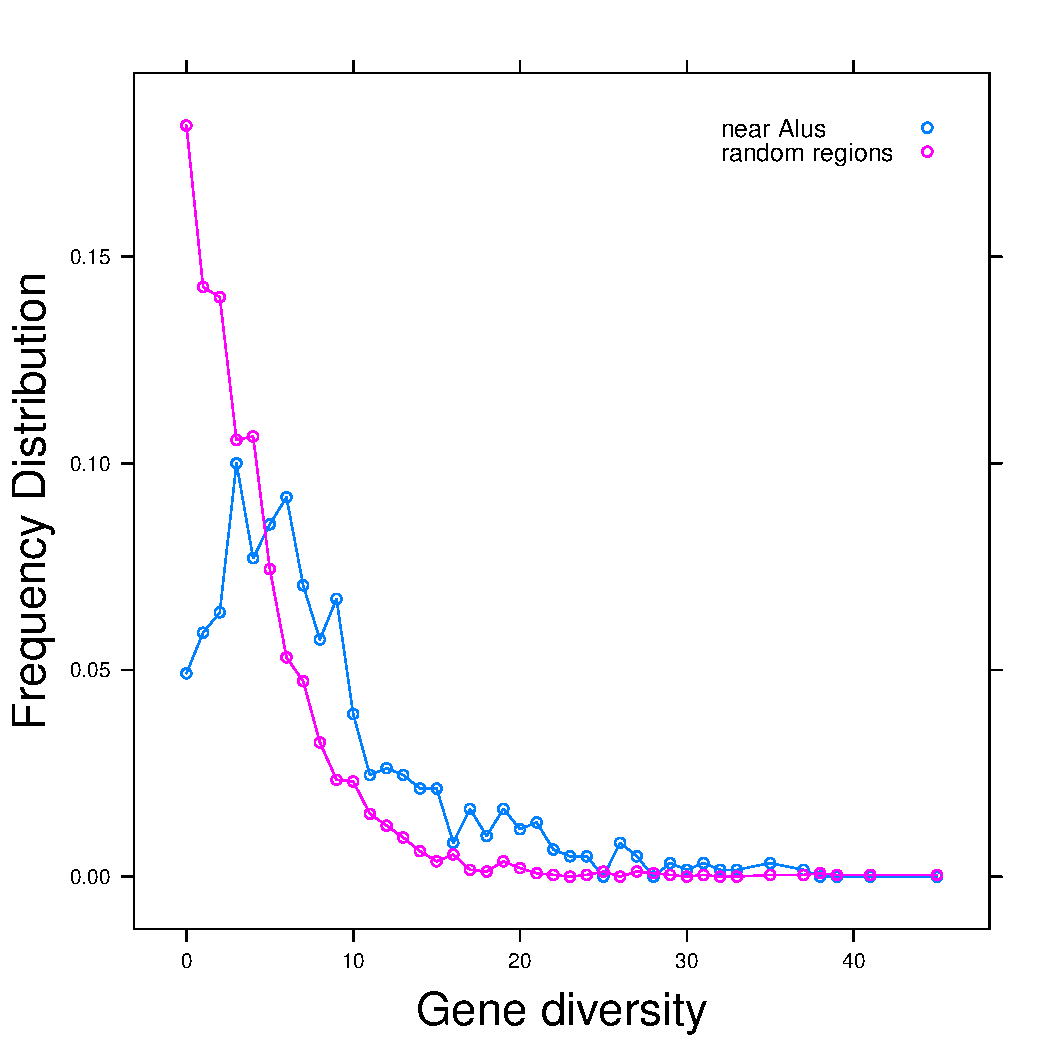
\includegraphics[height=0.8\textheight]{deeprand.pdf}\\ \scriptsize
Distributions are significantly different ($p\ll 10^{-30}$,
21X2 $\mathcal{X}^2$, Huff et al 2010).\\
\end{frame}


\begin{frame}
\frametitle{Genealogy of two genes}
{\centering
\mbox{\beginpicture
\setcoordinatesystem units <0.33\textwidth,0.2\textwidth>
%\setcoordinatesystem units <2cm,2cm>
\setplotarea x from 0 to 1.2, y from -0.1 to 1
%\axis bottom shiftedto y=-0.1
%  ticks withvalues {0} {$2N$} {$4N$} / at 0 1 2 / /
\arrow <1ex> [0.2,0.67] from 0.35 -0.15 to 0 -0.15
\arrow <1ex> [0.2,0.67] from 0.65 -0.15 to 1 -0.15
\put {$t_1$} at 0.5 -0.15
\put {$\bullet$} at 0 0
\put {$\bullet$} at 0 1
\plot 0 0 1 0 /
\plot 0 1 1 1 /
\plot 1 0 1 1 /
\plot 1 0.5 1.2 0.5 /
\endpicture}\\[10pt]}
$E[t_1] = 2N$~generations, where $N$ is effective population size.
\end{frame}

\begin{frame}
\frametitle{Hazards and lengths for a single pair of lineages}
\begin{columns}
\column[T]{0.48\linewidth}
Coalescent event: $h_c = 1/2N$
\column[T]{0.02\linewidth}
\pause
\rule{0.5pt}{0.6cm}
\column[T]{0.48\linewidth}
Mutation: $h_m = 2u$
\end{columns}
\pause
\noindent\rule{\linewidth}{0.5pt}

Hazard of an event of either type
\[
h = h_c + h_m = 1/2N + 2u
\]
\pause
\noindent\rule{\linewidth}{0.5pt}

Expected time until an event of either type
\begin{eqnarray*}
1/h &=& 1/(1/2N + 2u)\\
&=& \frac{2N}{1 + 4Nu}\\
&\approx& 2N \qquad\qquad\qquad \hbox{if $4Nu \ll 1$.}
\end{eqnarray*}
\end{frame}

\begin{frame}
\frametitle{Conditional on a single insertion}
\centering
\mbox{\beginpicture
\setcoordinatesystem units <0.33\textwidth,0.2\textwidth>
\setplotarea x from 0 to 2.2, y from -0.1 to 1
%\axis bottom shiftedto y=-0.1
%  ticks withvalues {0} {$2N$} {$4N$} / at 0 1 2 / /
\arrow <1ex> [0.2,0.67] from 0.35 -0.15 to 0 -0.15
\arrow <1ex> [0.2,0.67] from 0.65 -0.15 to 1 -0.15
\arrow <1ex> [0.2,0.67] from 1.35 -0.15 to 1 -0.15
\arrow <1ex> [0.2,0.67] from 1.65 -0.15 to 2 -0.15
\put {$t_1$} at 0.5 -0.15
\put {$t_2$} at 1.5 -0.15
\put {$\bullet$} at 0 0
\put {$\bullet$} at 0 1
\put {$\star$} at 1 1
\plot 0 0 2 0 /
\plot 0 1 2 1 /
\plot 2 0 2 1 /
\plot 2 0.5 2.2 0.5 /
\setdots
\putrule from 1 -0.15 to 1 1
\endpicture}\\

\bigskip

$E[t_1+t_2] \approx 4N$~generations.

\bigskip

Conditioning on insertion doubles length of genealogy (Tajima 1983).
\end{frame}

\begin{frame}
\frametitle{Nucleotide diversity decays with distance from Alu}
\centering
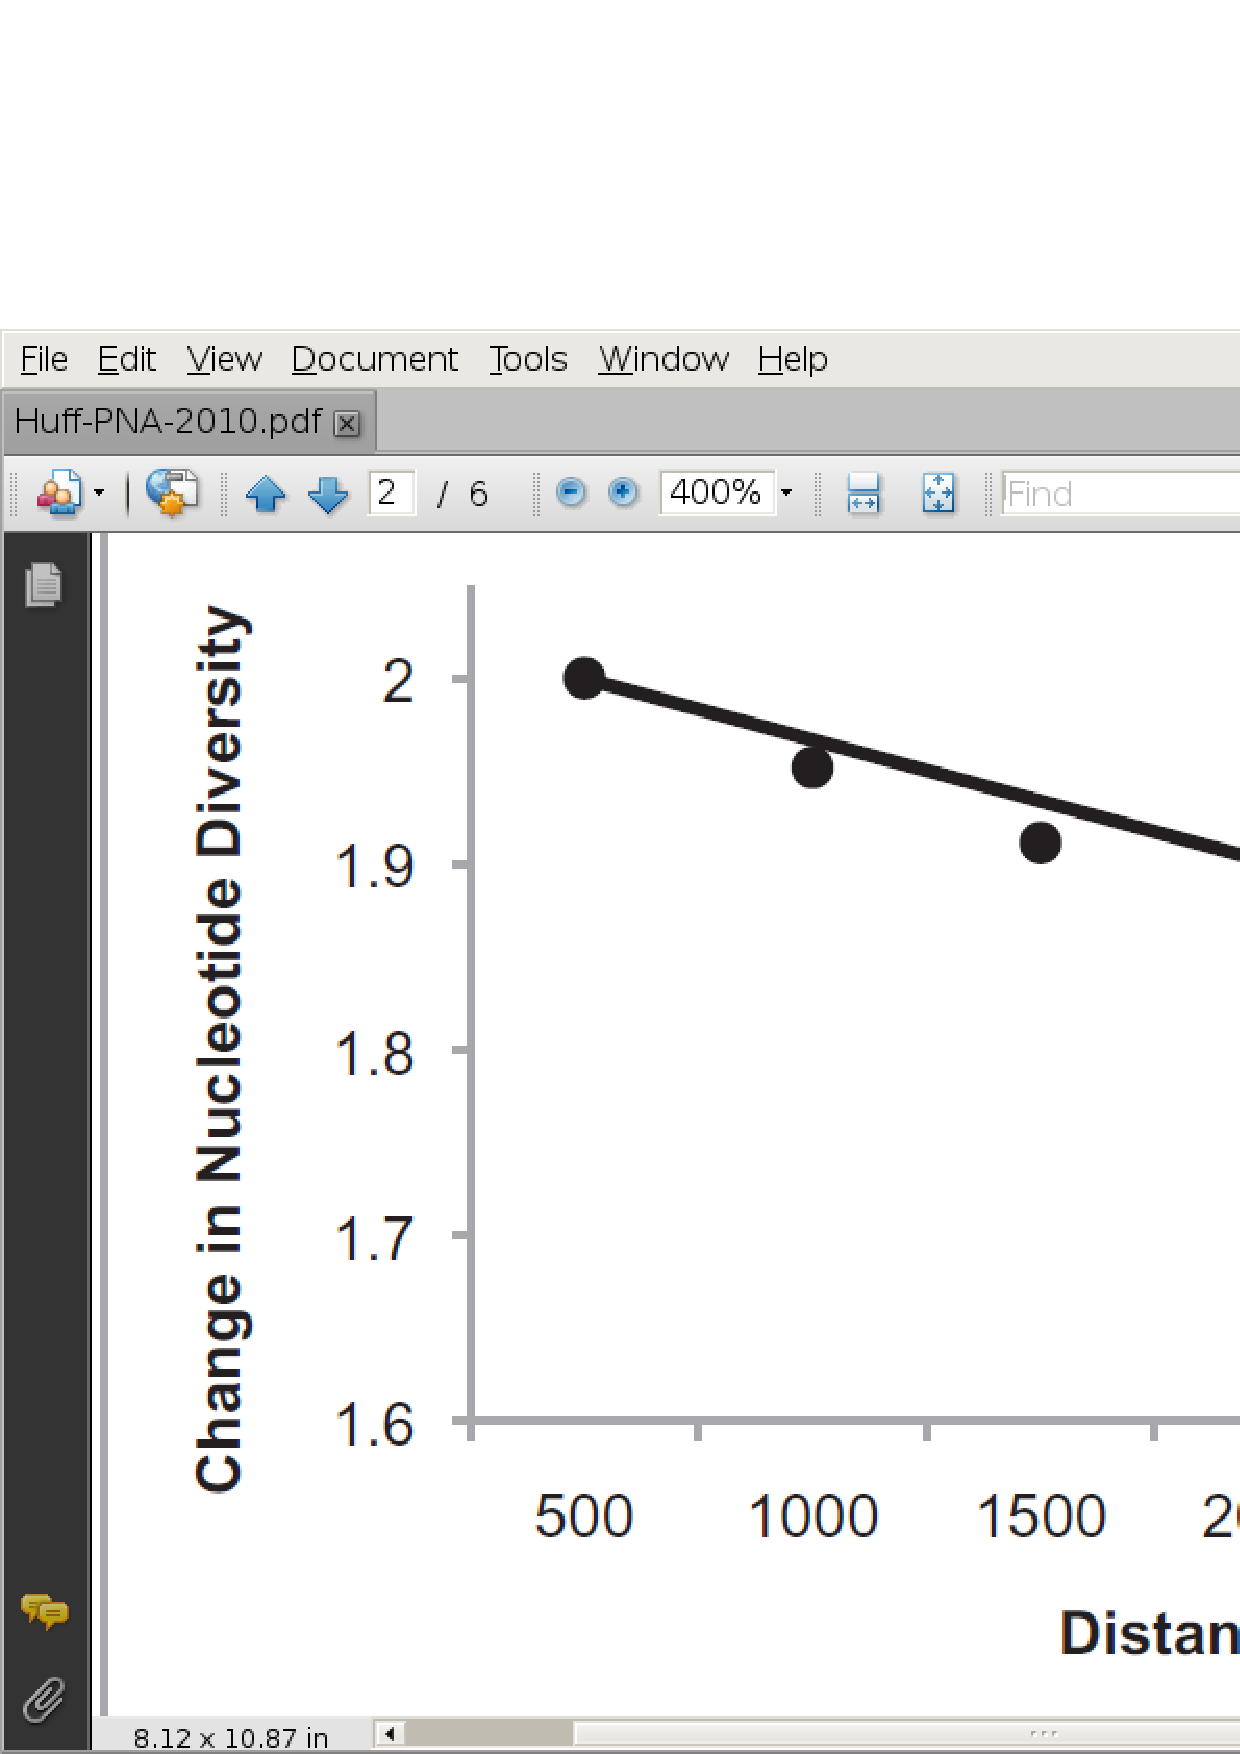
\includegraphics[width=\textwidth]{Huff-scatter.pdf}\\
{\mbox{}\hfill\footnotesize (Huff et al 2010)\\}
\pause
\bigskip
Can we use this to study history?
\end{frame}

\begin{frame}
\frametitle{Some hypotheses about population history}
\begin{center}
\includegraphics[height=0.85\textheight]{allhist-crop.pdf}\\
\end{center}
\end{frame}

\begin{frame}
\frametitle{Closeup of bottleneck}
\begin{columns}
\column{0.5\textwidth}
\includegraphics[width=\textwidth]{btlhist-crop.pdf}\\
\column{0.5\textwidth}
\begin{itemize}
\item Bottleneck is brief but severe.
\item Removes much of genetic variation.
\item Generates wave in mismatch distribution.
\end{itemize}
\end{columns}
\end{frame}

\begin{frame}
\frametitle{Data}
\begin{itemize}
\item Two complete genomes
\item 639 Alu insertions
\item DNA sequence variation w/i 2.5~kb of insertion, on either side
\item nucleotide diversity: fraction of sites that differ between two genomes.
\end{itemize}
\end{frame}

\begin{frame}
\frametitle{Statistical methods}
\begin{itemize}
\item Each hypothesis involves three parameters:
\begin{enumerate}
  \item Size $N_A$ of ancient population.
  \item Size $N_M$ of later population.
  \item Time $t$ since change in size.
\end{enumerate}
\item Simulate to approximate sampling distribution of gene diversity
  under each hypothesis.
\item Consider hypotheses covering a grid of $(N_A, N_M, t)$ values.
\item Likelihood ratio tests define confidence region.
\end{itemize}
\end{frame}

\begin{frame}
\frametitle{Quantile-quantile plots for random genomic regions}
{\centering
\includegraphics[height=0.85\textheight]{qqran-crop.pdf}\\}
\end{frame}

\begin{frame}
\frametitle{Quantile-quantile plots for regions near Alus}
{\centering
\includegraphics[height=0.85\textheight]{qqdeep-crop.pdf}\\}
\end{frame}

\begin{frame}
\frametitle{Point estimates and marginal confidence intervals}
\[
\begin{array}{rclc}
\hat t &=& 2.4      & (1.8{-}3)\\
\hat N_M &=& 17,000  & (16,200{-}17,500)\\
\hat N_A &=& 33,000 & (29,000{-}52,000)\\
\end{array}
\]
Using revised mutation rate, which is 1/2 as large as the one used by
Huff, 2010.

\bigskip\footnotesize

Ref: Huff, CD et al. 2010.  Mobile Elements Reveal Small Population
Size in the Ancient Ancestors of \emph{Homo sapiens}. PNAS 107(5):
2147--2152.
\end{frame}

\begin{frame}
\frametitle{Current research (Xing et al)}

Studied 4 genomes (2 European and 2 African) from the 1000-genomes
project.

\begin{center}
\begin{tabular}{lccc}
   & $t$ & $N_M$ & $N_A$\\
\hline
European  & 2.5 (2--2.8)   &  14,000 & 61,600 (43,400--70,000)\\
African   & 2.9 (2.5--3.3) &  15,500 & 57,400 (46,500--74,500)\\
\end{tabular}
\end{center}

\bigskip\footnotesize

Ref: Xing, Jinchuan, et al. In prep. Mobile elements demonstrate that
\emph{Australopithecus} effective size was twice that of \emph{Homo}.
(Used with permission.)
\end{frame}

\begin{frame}
\frametitle{SMC++: combines PSMC and spectrum (Terhorst, Kamm, \& Song 2017)}
\includegraphics[width=\textwidth]{Terhorst-pophist.jpg}
\end{frame}

\begin{frame}
\frametitle{Separation times (Terhorst, Kamm, \& Song 2017)}
\centering\includegraphics[height=0.8\textheight]{Terhorst-septime.jpg}\\
\end{frame}

\begin{frame}
\frametitle{Summary}
\begin{itemize}
\item Rare events provide a window into the distant past.
\item The human population declined 2--3~million years ago, at the
  origin of the genus \emph{Homo}.
\end{itemize}
\end{frame}

\end{document}
